\documentclass[10pt]{article}

\usepackage[english]{babel}
\usepackage[utf8x]{inputenc}
\usepackage{amsmath}
\usepackage{amssymb}
\usepackage{amsfonts}
\usepackage{graphicx}
\usepackage[ruled,linesnumbered,noend]{algorithm2e}
\usepackage{empheq}
\usepackage{float}
\usepackage{enumitem}
\usepackage{tikz}
\usepackage[colorlinks=true,urlcolor=blue]{hyperref}

\title{Introduction to Machine Learning, Fall 2014 - Exercise session III}
\author{Rodion ``rodde'' Efremov, student ID 013593012}

\begin{document}
 \maketitle

\section*{Problem 1 (3 points)}

\section*{Problem 2 (3 points)}

\section*{Problem 3 (3 points)}

\section*{Problem 4 (9 points)}
\subsection*{(a)}
\color{blue}
Download the MNIST data from the course web page. In addition to the actual data, the package contains some functions for easily loading the data into Python/Matlab/Octave/R and for displaying digits. See the README files for details. Load the first $N=5,000$ images using the provided function.
\color{black}

\subsection*{Solution to (a)} 
Check!

\subsection*{(b)}
\color{blue}
Use the provided functions to plot a random sample of 100 handwritten digits, and show the associated labels. Verify that the labels match the digit images. (This is a sanity check that you have the data [is] in the right format.)
\color{black}

\subsection*{Solution to (b)}
\begin{center}
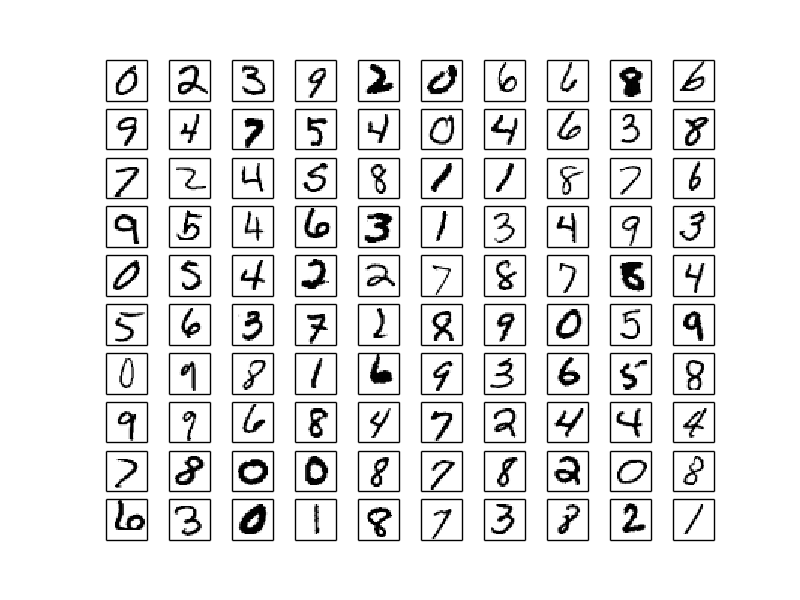
\includegraphics[scale=0.5]{100TestMnistImages}
\end{center}
The labels are:
\begin{center}
\begin{verbatim}
0 2 3 9 2 0 6 6 8 6 
9 4 7 5 4 0 4 6 3 8 
7 2 4 5 8 1 1 8 7 6 
9 5 4 6 3 1 3 4 9 3 
0 5 4 2 2 7 8 7 8 4 
5 6 3 7 2 8 9 0 5 9 
0 9 8 1 6 9 3 6 5 8 
9 9 6 8 4 7 2 4 4 4 
7 8 0 0 8 7 8 2 0 8 
6 3 0 1 8 7 3 8 2 1
\end{verbatim}
\end{center}

\subsection*{(c)}
\color{blue}
Divide the data into two parts: A `training set` consisting of the first 2,500 images (and associated labels), and a `test set` containing the remaining 2,500 images (and their associated labels).
\color{black}

\subsection*{Solution to (c)}
Check!

\subsection*{(d)}
\color{blue}
For each of the ten classes (digits 0-9), compute a class \textit{prototype} given by the mean of all the images in the training set that belong to this class. That is, select from the training set all images of class '0' and compute the mean image of these; this should look sort of like a zero. Do this for all ten classes, and plot the resulting images. Do they look like what you would expect?
\color{black}

\subsection*{Solution to (d)}
\begin{center}
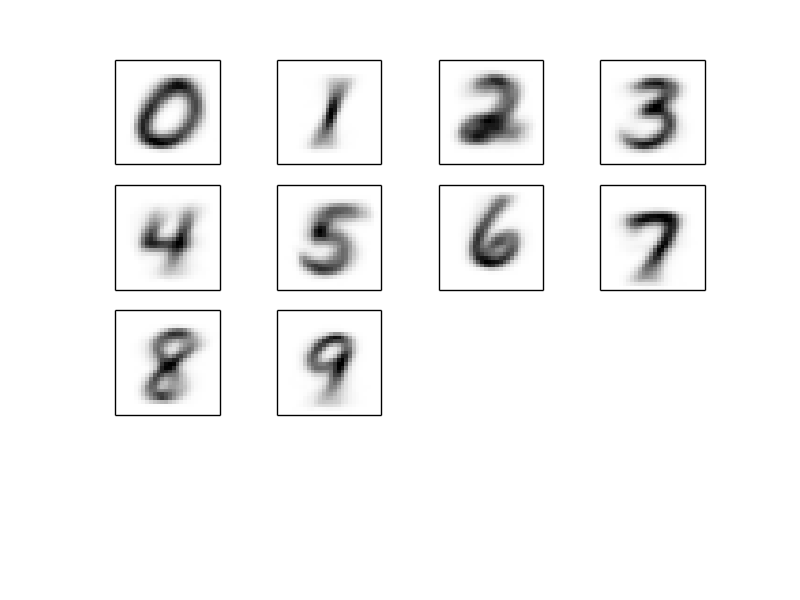
\includegraphics[scale=0.5]{MNISTPrototypes}
\end{center}
Obviously, the prototypes look good.
\end{document}